\chapter{Stato dell'Arte}

In un contesto complesso, dinamico e spesso riservato come quello di un pronto soccorso, può risultare molto arduo ottenere informazioni volte a realizzarne una rappresentazione, seppur in forma modellare, che si avvicini il più possibile al sistema reale. 
 
Per questo motivo è spesso utile per un modellista basarsi su quello che è chiamato lo \textit{``stato dell'arte"}: articoli scientifici, libri e strumenti che descrivono il massimo livello di sviluppo nella ricerca in un determinato ambito. 

Nel caso in esame, abbiamo deciso di basarci sul lavoro di diversi ricercatori che avessero già approfondito il tema, tramite progetti riportati sotto forma di paper scientifici.  

\section{Paper}

Gli articoli scientifici su cui si è basato il nostro modello sono i seguenti:
\begin{itemize}
\item \cite{garcia_reducing_1995}
\item \cite{espinoza_real-time_2014}
\item \cite{stainsby_towards_2009} 
\item  \cite{wang_agent-based_2009}
\end{itemize}


Il lavoro svolto in ciascuna di queste ricerche è servito principalmente a non dover sviluppare un nuovo modello partendo da zero: è risultato infatti difficile ottenere informazioni direttamente sul campo, a causa della riservatezza caratteristica dell'ambiente in oggetto. 

In particolare, i paper \textit{\cite{garcia_reducing_1995}}, \textit{\cite{stainsby_towards_2009}} e \textit{\cite{wang_agent-based_2009}} sono risultati utili a definire un workflow (vedi \textit{Capitolo 4}) che potesse dare forma all'interazione degli agenti con l'ambiente, ai percorsi seguiti e alle risorse utilizzate.

\begin{figure}[!htb]
    \centering
    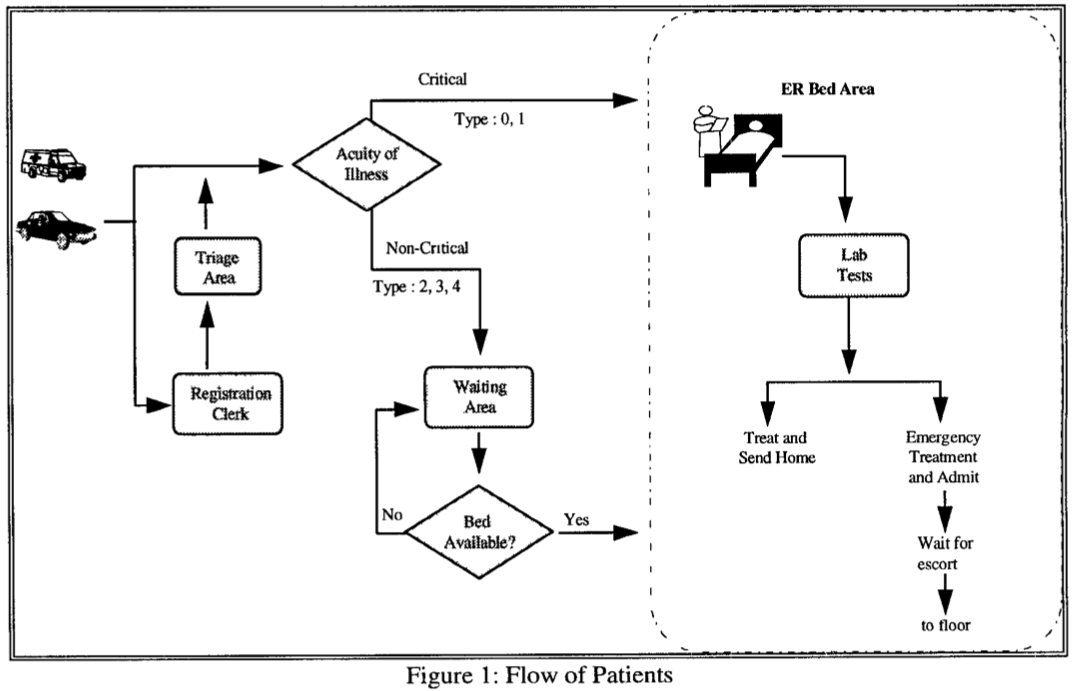
\includegraphics[width=1\textwidth]{Immagini/garcia-wf.png} 
    \caption{Workflow utilizzato nel paper \textit{\cite{garcia_reducing_1995}}}
\end{figure}

\begin{figure}[!htb]
    \centering
    \makebox[\textwidth][c]{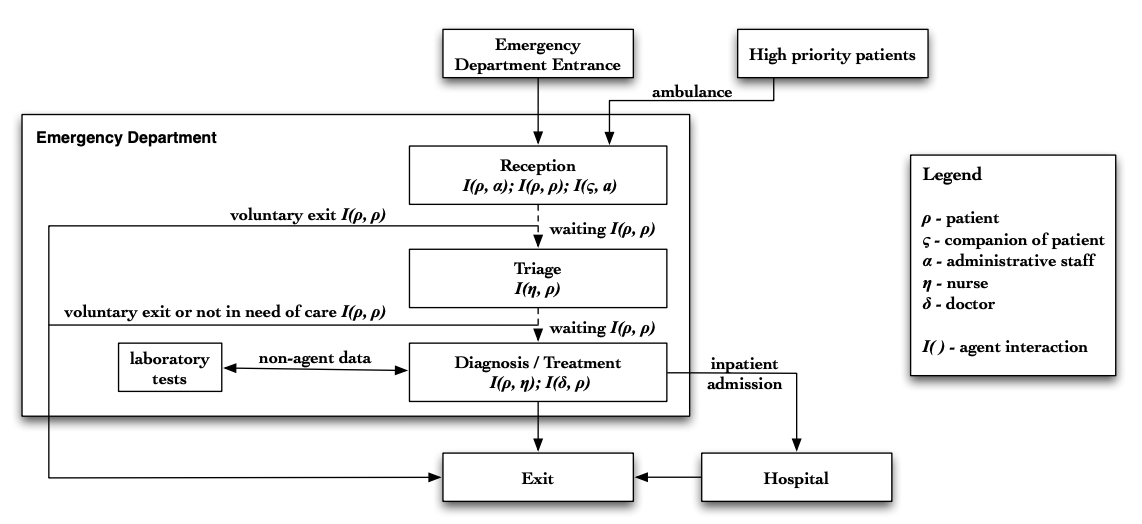
\includegraphics[width=1\textwidth]{Immagini/stainsby-wf.png}}   
    \caption{Workflow utilizzato nel paper \textit{\cite{stainsby_towards_2009}}}
\end{figure}

\begin{figure}[!htb]
    \centering
    \makebox[\textwidth][c]{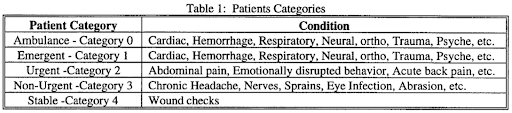
\includegraphics[width=1\textwidth]{Immagini/garcia-priority.png}}   
    \caption{Codici di priorità utilizzati nel paper \textit{\cite{stainsby_towards_2009}}}
\end{figure}

\begin{figure}[!htb]
    \centering
    \makebox[\textwidth][c]{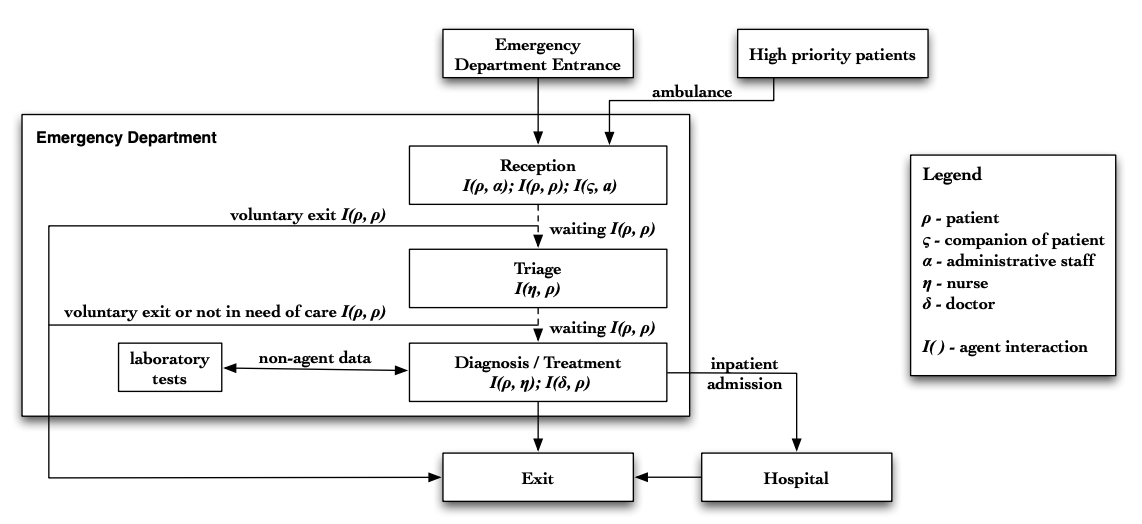
\includegraphics[width=1\textwidth]{Immagini/stainsby-wf.png}}   
    \caption{Codici di priorità reperibili dal sito della \textit{Regione Lombardia}}
\end{figure}

Il paper \textit{\cite{espinoza_real-time_2014}} è servito a definire delle metriche per effettuare sperimentazioni e a confrontarne i risultati con quelli ottenuti nei lavori precedenti (vedi \textit{Capitolo 5}). 

Infine, consultando nuovamente il paper \textit{\cite{garcia_reducing_1995}} e confrontandolo con le informazioni riportate sul sito della \textit{Regione Lombardia} (per un maggiore adattamento a quello che è il modello locale), è risultato possibile ottenere una rappresentazione tabellare della gravità tipica dei pazienti ed annessa priorità. 


\clearpage
\section{Strumenti}

Per completare l'approfondimento relativo a quello che è lo stato dell'arte, in questa sezione verranno descritti brevemente gli strumenti utilizzati in ciascuno dei paper consultati. 

È doveroso riportare che solo in uno di questi lavori non è stata effettuata una simulazione né sono stati adoperati strumenti informatici di supporto: in particolare, nel paper \textit{\cite{stainsby_towards_2009}} è stato realizzato unicamente il modello matematico per il raggiungimento di un modello ad agenti simulabile (il titolo recita ``\textit{towards}", per l'appunto).

\subsection{Garcia et al., 1995: \textit{SIMAN}}

Lo strumento utilizzato in questo paper per simulare il modello è un linguaggio chiamato SIMAN (SIMulation ANalysis), presentato nel 1982 nell'articolo \textit{\cite{pegden_simulation_1982}}. 

È utilizzato per modellare sistemi combinati discreto-continui, tramite l'impiego di diversi approcci: per il discreto, si orienta verso l'utilizzo di \textit{processi} oppure \textit{eventi}. 
La parte continua è modellata tramite \textit{algebra, differenze} o \textit{equazioni differenziali}. 


\subsection{Espinoza et al., 2014: \textit{FlexSim HC}}

FlexSim HC (HealthCare) è un ambiente di simulazione sviluppato da FlexSim, adoperato  a livello aziendale nell'ambito della salute. 
In maniera simile ad AnyLogic, permette di modellare un ambiente 3D ed un workflow per orientare pazienti e staff all'interno del detto ambiente. 

Sul \underline{\href{https://www.flexsim.com/healthcare/flexsim-hc/}{sito Internet dedicato}} è possibile scaricarne una versione di prova gratuita per testarne le funzionalità. 

\subsection{Wang, 2009: \textit{NetLogo}}

NetLogo è un linguaggio di programmazione e IDE per la modellazione basata su agenti. 
Presentato nel 1999, è particolarmente efficace per l'esplorazione di \textit{fenomeni emergenti}, di cui include una vasta libreria di modelli al suo interno. 

NetLogo è open-source e scaricabile gratuitamente dal \underline{\href{http://ccl.northwestern.edu/netlogo/}{suo sito Internet}}. 





